\documentclass[12pt]{article}
%%%%%%%%%%%%%%%%%%%%%%%%%%%%%%%%%%%%%%%%%%%%%%%%%%%%%%%%%%%%%%%%%%%%%%%%%%%%%%%%%%%%%%%%%%%%%%%%%%%%%%%%%%%%%%%%%%%%%%%%%%%%%%%%%%%%%%%%%%%%%%%%%%%%%%%%%%%%%%%%%%%%%%%%%%%%%%%%%%%%%%%%%%%%%%%%%%%%%%%%%%%%%%%%%%%%%%%%%%%%%%%%%%%%%%%%%%%%%%%%%%%%%%%%%%%%
\usepackage{amsfonts}
\usepackage{eurosym}
\usepackage{geometry}
\usepackage{amsmath,amsthm,amssymb}
\usepackage{graphicx}
\usepackage{comment}
%\usepackage[sort,comma]{natbib}
\usepackage[backend=biber, style = apa]{biblatex}
\usepackage{placeins} % to separate sections

\usepackage{adjustbox}
\usepackage{array}
\usepackage{multirow}
\usepackage{graphicx}
\usepackage{subcaption}
\usepackage{pifont}
\usepackage{amssymb}
\usepackage{comment}
\usepackage[utf8]{inputenc}
\usepackage{setspace}
\usepackage[hang, flushmargin, bottom]{footmisc}
\usepackage{footnotebackref}
\usepackage{xcolor}
\usepackage{hyperref}
\usepackage{booktabs}
\usepackage{pifont}
\usepackage{caption}
\usepackage{float}
\usepackage{todonotes}
\setcounter{MaxMatrixCols}{10}
%TCIDATA{OutputFilter=LATEX.DLL}
%TCIDATA{Version=5.50.0.2960}
%TCIDATA{<META NAME="SaveForMode" CONTENT="1">}
%TCIDATA{BibliographyScheme=BibTeX}
%TCIDATA{LastRevised=Sunday, April 28, 2024 18:12:38}
%TCIDATA{<META NAME="GraphicsSave" CONTENT="32">}
%TCIDATA{Language=American English}

%\setlength{\bibsep}{0.3pt}
\setlength{\textfloatsep}{5pt}
\hypersetup{breaklinks=true,hypertexnames=false,colorlinks=true,citecolor = teal}
\captionsetup{font=normalsize}
\newcommand{\cmark}{\ding{51}}
\def\sym#1{\ifmmode^{#1}\else\(^{#1}\)\fi}
\renewcommand{\thetable}{\Roman{table}}
\geometry{verbose,tmargin=1.252in,bmargin=1.252in,lmargin=1.2in,rmargin=1.2in,nomarginpar}
\makeatletter
\DeclareTextSymbolDefault{\textquotedbl}{T1}
\theoremstyle{plain}
\newtheorem{thm}{\protect\theoremname}
\theoremstyle{plain}
\newtheorem{prop}[thm]{\protect\propositionname}
\providecommand{\propositionname}{Proposition}
\providecommand{\theoremname}{Theorem}
\makeatother
\providecommand{\propositionname}{Proposition}
\providecommand{\theoremname}{Theorem}
\newtheorem{ass}[thm]{Assumption}
% \input{tcilatex}
\usepackage{tikz}
\usetikzlibrary{shapes.geometric, arrows, positioning}

\tikzstyle{startstop} = [rectangle, rounded corners, minimum width=3cm, minimum height=1cm, text centered, draw=black, fill=blue!30]
\tikzstyle{process} = [rectangle, minimum width=3cm, minimum height=1cm, text centered, draw=black, fill=orange!30]
\tikzstyle{decision} = [rectangle, minimum width=3.5cm, minimum height=1cm, text centered, draw=black, fill=red!30]
\tikzstyle{mechanism} = [rectangle, minimum width=3cm, minimum height=1cm, text centered, draw=black, fill=green!30]
\tikzstyle{arrow} = [thick,->,>=stealth]



\addbibresource{references.bib}
\begin{document}
 

\newpage
 \title{{\Large Centralized annuities marketplace}}
\author{Lucas Schmitz\thanks{Yale University \texttt{lucas.schmitz@yale.edu}}} 
\date{}
\maketitle


%

%\begin{abstract}
%\baselineskip0.5cm Here goes the abstract.
%\end{abstract}

%\thispagestyle{empty}

\vspace{3cm}

%\newpage \onehalfspacing
%\setcounter{page}{1}

\begin{abstract}
\end{abstract}

\vspace{2cm}
\section{Introduction}




\section{Institutional Context and Data}\label{sec: context and data}

 This description of the institutional context heavily relies on the description by \textcite{boehm_intermediation_2024}.

Chile operates a fully funded, defined-contribution pension system. Throughout their working lives, individuals are required to contribute 10\% of their wages to a personal retirement account. These accounts are managed by private Pension Fund Administrators (PFAs), who invest the funds in a mix of equities, bonds, and mutual funds. Upon reaching retirement age — 65 for men, 60 for women, or earlier in cases of sufficient accumulated wealth or disability — individuals must convert their savings into a stream of retirement income by selecting a pension product. Retirees are generally not allowed to make lump-sum withdrawals.


\textbf{Pension products} Retirees opting for a Phased Withdrawal (PW) maintain their savings accounts under PFA management and make systematic withdrawals based on an actuarial formula set by the government. The withdrawal amount is updated annually, reflecting factors such as life expectancy based on a national mortality table, expected returns on investment, and the presence of any dependents (spouses or children under 24 years old). Under this arrangement, retirees retain ownership of their remaining savings, which can be passed on as an inheritance if they die prematurely. However, they bear the risk of outliving their savings, as pension payments decline over time until the account is depleted\footnote{If the pension falls below a threshold the government tops it up, which creates a distortion between the PW and the annuity because in the later case there is no government subsidy. The government also insures 75\% of the worker’s annuity over the MPG (with a cap of 45UF or about US\$1200 monthly) in case the insurance company becomes insolvent, and to prevent this from happening sets stringent reserve, equity and asset-liability matching requirements. So far it has never had to pay this insurance(\cite{james_pensiones_2005})}. Retirees under PW are also exposed to fluctuations in interest rates, leading to potential volatility in the value of their pension savings.

As an alternative to the Phased Withdrawal, the retiree can purchase an annuity from an insurance company. This choice entails the individual giving up ownership of their savings in exchange for longevity insurance: the insurance company contracts an obligation to pay a fixed, inflation-adjusted amount for the remaining duration of the retiree’s lives. The retiree therefore transfers their longevity risk to the insurance company but gives up the possibility of bequeathing part of their pension savings.

Retirees have the ability to tailor their annuity contracts, particularly by selecting guarantee and deferral options. A guarantee period ensures that the annuity will continue to make payments for a minimum period, offering some protection against early death while still allowing for a potential bequest. Retirees can also allocate a portion of their savings to purchase a deferred annuity, using the remaining balance to increase initial payouts. It is possible to combine guarantee and deferral features within a single contract.

To assist with decision-making, retirees can request and receive multiple quotes through a centralized exchange platform (SCOMP), ultimately choosing among options listed in a document known as the Offers Certificate. The typical retiree requests quotes for around 10 different product types and receives more than 100 quotes overall.
The range of available pension products involves inherent trade-offs among securing higher initial payments, insuring against longevity risk, and preserving wealth for heirs. Thus, selecting the optimal pension product depends critically on how product features interact with an individual's expected lifespan, desire to leave an inheritance, risk tolerance, and degree of impatience. Reaching a well-informed decision requires not only an understanding of financial concepts and contract terms but also a careful reflection on personal preferences, anticipated longevity, and the retiree’s broader financial circumstances. Given the complexity of these considerations and the documented gaps in financial literacy regarding pensions, this decision-making process can be both challenging and cognitively demanding for retirees.



\textbf{Centralized exchange}

By regulation, the process that leads to the purchase of an annuity takes place in SCOMP.  Established in 2004, SCOMP was designed to enhance retirees' access to information about their available options and to simplify the process of obtaining and comparing offers from various insurance companies and PFAs (CMF, 2019). Individuals who have accumulated savings above a minimum threshold can request quotes for annuities with different combinations of guarantee and deferral periods. These quote requests are circulated to all insurance companies active in the market, accompanied only by basic information: the retiree’s age, gender, marital status, the age of any legal beneficiaries, and the total amount of savings. Each insurer then decides whether to respond with a quote for each requested pension product.

 
 

 All offers — including Phased Withdrawal offers from PFAs and annuity offers from insurance companies — are compiled into a  document called the Offers Certificate, which is mailed to the retiree. All quotes must be stated in "UF," an inflation-indexed unit of account, ensuring that annuity values are presented in real terms. Figures \ref{fig:offer_PW} and \ref{fig:offer_ann2} illustrate the payments under a Phased Withdrawal and the range of annuity offers for a given year, while Figure \ref{fig:offer_ann2} displays offers for another year. Retirees also receive information about the risk rating assigned to each insurance company, an important consideration since retirees are only partially protected in the event of insurer insolvency. The median retiree requests quotes for 10 product types and receives over 100 quotes for pension products.  



Once they receive the Offers Certificate, retirees can either accept one of the offers, postpone their decision, or attempt to negotiate directly with insurance companies to improve an existing offer. To negotiate, retirees must physically visit the branch of the insurance company. It is important to note that firms are prohibited from offering worse terms during this stage. On average, negotiated offers improve the initial terms modestly, with increases of around 2\% in generosity compared to the original SCOMP offers (\cite{illanes_retirement_2019}).

\textcolor{red}{from here on is a copy of the institutional description of boehm }

 The number of retirees using SCOMP has increased through time, reaching over 50, 000 in 2018, at which point the annual value of the pension market was over 6 billion dollars . From 2004 onwards, 19 insurance companies have participated in the annuity market. For a majority of them, annuities constitute an important business line, making up over 60\% of both revenues and liabilities. Insurance companies are differentiated by their risk rating, an evaluation of their creditworthiness assessed periodically by two independent agencies. The regulator explicitly forbids the bundling of pension products with other types of insurance. Nevertheless, insurance companies might also differ in terms of their customer service, office locations and brand appeal.


\begin{figure}
    \centering
    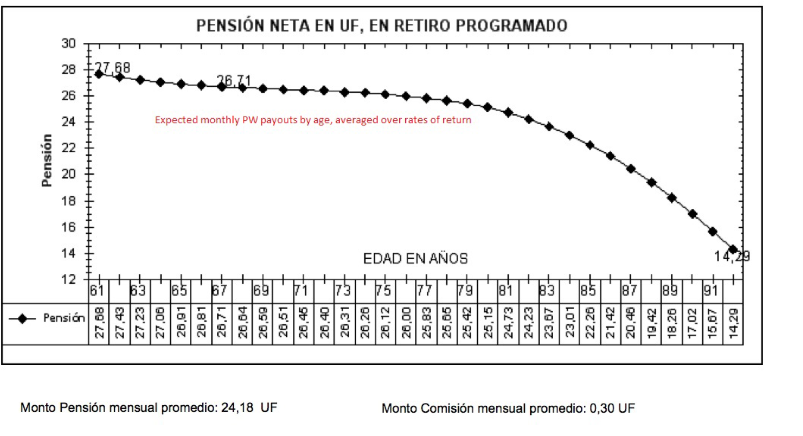
\includegraphics[width=0.5\linewidth]{figures/PW_flows.png}
    \caption{Payments under PW (source \textcite{illanes_retirement_2019}}
    \label{fig:offer_PW}
\end{figure}

\begin{figure}
    \centering
    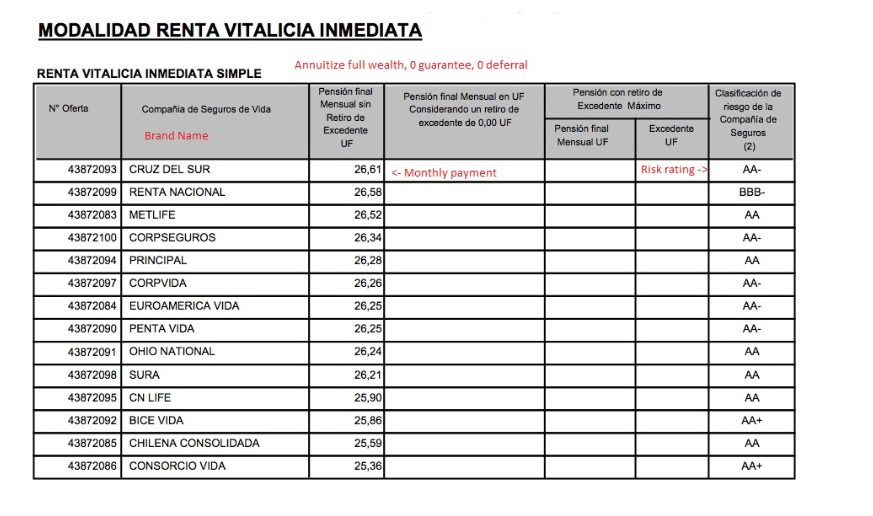
\includegraphics[width=0.5\linewidth]{figures/annuity_offer.png}
    \caption{Annuity offer (source \textcite{illanes_retirement_2019}}
    \label{fig:offer_ann1}
\end{figure}

\begin{figure}
    \centering
    
\includegraphics[width=0.5\linewidth]{figures/offer_certificate.png}
    \caption{Annuity offer (source \textcite{boehm_intermediation_2024}}
    \label{fig:offer_ann2}
\end{figure}

\vspace{3cm}
\subsection{Policy variation}
\begin{itemize}
    \item \
\end{itemize}
\textcolor{red}{what has been the policy variation since 2004? }

\textcite{alcalde_intermediary_nodate} study a refore where: \textit{
Before the reform, both intermediaries received a commission of 2.5\% of the retiree’s retirement fund if the customer chose an annuity but no commission for programmed withdrawal. Advisers took payment in any event, but sales agents only got paid if the annuity came from his firm, and thus average commissions were lower for sales agents. The reform reduced the commission for annuities to 2\%, with a cap of approximately US\$2,500, starting in October 2008. Later, it introduced a commission—only for advisers— of 1.2\% for programmed withdrawal, with a cap of approximately US\$1,500, beginning in April 2009.}



For a description of credit ratings and the risk of insurance companies see the \textcite[p.5]{aryal_auctioning_2021}

For descriptive statistics tables see \textcite{aryal_auctioning_2021}
\textcolor{red}{describe how beneficiaries are paired with brokers-intermediaries.} 

For a motivation of what the SCOMP aimed to achieve and for further reforms after the 2004 reform see \textcite[section 3.2]{halcartegaray_efectos_2011}. 

\subsection{Curious facts}

\begin{itemize}
    \item In the US the MWR of contracts is in the range .7-.85 (\cite{noauthor_lecture_annuities_nodate}) whereas in Chile they are greater than 1 (\cite{quiroz_estudio_2018}). 
    \item 31\% of annuities in 2017 were for women and 69\% for men 
\end{itemize}

%%%%%%%%%%%%%%%%%%%%%%%%%%%%%%%%%
%%%%%%%%%%%%%%%%%%%%%%%%%%%%%%%%%
\section{Data}
There are already a couple of papers that have studied this market (\cite{boehm_intermediation_2024,illanes_retirement_2019,alcalde_intermediary_nodate} the data sources we could use are: 

\begin{itemize}
    \item The first one is the centralized offer exchange database SCOMP, available from the regulating agencies, which contains all retirees from August 2004 until July 2020. This database includes basic demographic information about retirees – age, gender, and legal dependents – total savings, geographic location at the city/precinct level. The data also record every offer received by each potential retiree, information about intermediation, pension product accepted, and commission paid. Finally, I also observe the date of death if it occurs before July 2021. I complement this information with publicly available reports on insurance companies’ risk ratings, information about the number of intermediaries, and their registered locations. For a subset of the independent advisors, I also link scores obtained in the knowledge tests required for their certification after 2017. For most of the analysis, I restrict the sample to individuals retiring between 2010 and 2018, at or after legal age, and without legal dependents other than a spouse. This sample selection yields approx. 150,000 observations.

    \item Administrative database of Pension Histories (HPA) from the Superintendence of Pensions.(\cite{halcartegaray_efectos_2011}) 
    
    \item Aggregate time series data on annuities and programmed withdrawals for normal old age and early retirement, 1983-2002, were obtained from the insurance regulator and the AFP regulator (\cite{james_pensiones_2005}.
    
    \item Individual-level data on all annuitants giving gender, size of pensions and dates of birth, retirement and death. (Unfortunately, comparable data on programmed withdrawal pensioners were not available) (\cite{james_pensiones_2005}). 
    
    \item Annuity quotes from several companies for 2003 and 1999, from which we calculated money’s worth ratios (\cite{james_pensiones_2005}). 


\item \textbf{Surveys: } The firs one is the Social Protection Survey, a representative panel survey conducted by the Department of Social Protection in Chile. Individuals are periodically interviewed on work history, education, health, income, wealth, and information regarding social security, pensions, and their knowledge of the system. The second survey conducted as part of the choice-architecture experiment of Duch et al. (2021), who elicit information about soon-to-be retirees’ income, education level, financial literacy, risk preferences, and their plans for retirement. The survey also asks about preferences for different pension products after conducting an information intervention about their characteristics

\item \textcolor{red}{What is the data that we have from before the SCOMP? }

\end{itemize}

The great advantage of the setting and associated data is that 1. we observe the non-selected offers and 2. the consumer observes all the offers. If the market is not centralized the consumer might not request a quote from every single insurer, whereas here they request one quote and all the insurers bid, and also even when the consumer requests multiple quotes, if the data only includes realized transactions, the quotes will not be observed by the econometrician. Whereas most models of insurance markets (Akerloff 70 \& Roth. and Stiglitz 76) model a perfectly competitive insurance market we allow for differentiation. 


\section{Motivation}

\begin{itemize}
    \item To increase the annuitization rate \textcite{benartzi_annuitization_2011} propose: 
    \begin{enumerate}
        \item  An alternative strategy would be to make the annuity products safer via a government guarantee along the lines of the Federal Deposit Insurance Corporation  for banks and the Pension Benefit Guaranty Corporation for pension plans.   
        \item " increasing the supply of easy-to-find annuity options for those of retirement age with 401(k) and other defined contribution plans.  The goal should be to emulate the progress that has taken place during the last two decades in the design of plans for the accumulation taken place during the last two decades in the design of plans for the accumulation phase: specifically, the widespread adoption of “automatic” features, including automatic enrollment, automatic escalation, and default investment strategies such as “target date funds” that rebalance a portfolio for a decreasing level riskiness as the participant ages."
        
    \end{enumerate}
    with respect to the first proposal, our setting allows us to directly estimate the increase in consumer welfare that a government guarantee would generate and the impact on the annuitization rate. NOT CLEAR WHAT DO WE HAVE TO SAY WRT THE SECOND PROPOSAL, MAYBE WE COULD SAY SOMETHING ELSE IF WE GET DATA FROM THE SYSTEM PRIOR TO SCOMP. 
    
\end{itemize}

Other aspects that are interesting of our context is that in standard models of insurance markets firms compet either in price (Akerlof 70) or price and coverage (Rothschild and Stiglitz 76). In our case consumers by choosing the number of guaranteed periods can themselves determine something akin to the coverage, which changes the way firms compete.  


There are a couple of other markets where sellers post a price and then the buyer can bargain with the seller, e.g. car dealerships and the housing markets where if you go to Zillow you have a price but you can always contact the seller to get a better price. The difference is that in those markets the buyer has less information than the seller whereas in our case is the opposite.  

\section{Research questions}

\begin{itemize}
    \item One of the big questions is why is it that people do not buy more annuities. But one has to consider they are not backed, there is a risk the insurance company goes bankrupt\footnote{The government reinsures a minimum pension plus 75\% of the difference between the annuity payment and the minimum, up to a cap of 45 UFs. There has been only one bankruptcy since the system’s introduction in the 1980s, and that company’s annuitants received their full payments for 124 months after bankruptcy.(\cite{illanes_retirement_2019})}. This setting is particularly well suited to see how much people value the credit risk of the companies since one observes all the offers \footnote{In normal contexts might be difficult to observe the choice set of the individuals}. Here one could 1. see how much people value decreases in the insurers risk and simulate take up in a case where there is no insurer risk at all. 

    \item A classical problem in insurance markets is that adverse selection might generate unraveling (\cite{rothschild_equilibrium_1976})\footnote{Contracts in the \textcite{rothschild_equilibrium_1976} model have two dimensions: premiums and coverage, in annuities contracts are uni-dimensional. We are not sure about the implications of this distinction.}. Moreover a long-standing puzzle in finance is the low share of the population who buys annuities (\cite{modigliani_life_1986}), since under a broad range of assumptions models predict annuitization. This issue is particularly salient in the Chilean insurance market where the money worth's ratio \footnote{The Money Worth's ratio denotes the ratio of expected present value of insurance payments divided by the price of the insurance contract.} is greater than 1. A possible policy intervention is to make it mandatory to buy the annuities. There are two research questions related to this policy 1. is there adverse selection? (\cite{chiappori_testing_2000, einav_estimating_2010}) and 2. what are the welfare gains from a mandatory annuities purchase? 

    \begin{itemize}
        \item \textcite{einav_selection_2011} say "The canonical solution to the inefficiency created by adverse selection is to mandate that everyone purchase insurance."

        \item \textcite{illanes_retirement_2019} already study this issue. 
    \end{itemize}

    \item Before the 2004 reform that created SCOMP comissions reached an average of 6\% with fees for particular transactions as high as 11\% (\cite[p. 390]{morales_chilean_2017}. The 2004 reform increased competition by making the system more transparent, and at the same time it capped comissions to 2.5\% (\cite[p. 391]{morales_chilean_2017}), what were the impacts of this? Normally if you cap comissions in a market you decrease access, but probably is not the case if there is some behavioral bias. The answer could provide information of what happens when you decrease search costs\footnote{For example \textcite{cannon_price_2015} finds huge returns to searching. But is not very well published, although I would expect to see more papers showing that the estimated search costs (equivalently the returns of searching) are huge }.  Maybe SCOMP coul also be linked to the idea of bargaining vs auctions, is it better to have SCOMP (auction system) or allow the beneficiaries to bargain? 

    \begin{itemize}
        \item A solution to the annuitization puzzle proposed by \textcite{benartzi_annuitization_2011} is that people do not buy annuities because is not the default. They mention some difficulties (making a call) as the explanation of low 401k enrollment and this could also be the case with annuities\footnote{They say "\textit{Much research shows that even tiny obstacles such as the need to make a phone call or fill in a form can result in  procrastination and lack of action in a retirement savings plan. .... 
        The same issues apply to the choice of whether to annuitize. Is the low annuitization rate a reflection of underlying preferences or of features of the choice environment? This question has important practical implications, because in most retirement plans when an employee stops working, that retiree would have to shop  around actively if interested in investing some or all of the retirement plan balance in an annuity. Remember, few defined contribution plans offer annuities.  Owners of Individual Retirement Accounts (IRAs) are in the same boat; they have to seek out  annuity products as they reach retirement if they want to ensure lifetime income.}"}. By studying the impact of centrlaizing SCOMP we would be able to provide evidence to back or reject this argument. They even speak about cases where people actively choose between PW and annuity as a context where to study their claims (p. 150-152). 
    \end{itemize}

    \item A question is what are the effects of having an aftermarket where you can bargain with sellers, when you already have posted prices. There are a couple of other situations where this happen 
    \begin{enumerate}
        \item Charles mentioned in our meeting (18june25) that since centralized insurance markets are used in many places understanding whether the aftermarket is good or bad seems to be super important. Apparently in the UK you can get some particular health insurance conditional on getting an exam.
    \end{enumerate}
    
\end{itemize}

\section{Model}
Our model presents some particularities from the standard model of consumers buying goods:
\begin{itemize}
    \item Prices are individualized, insurers take into account the  risk
\end{itemize}

\textbf{Demand model}
 
Individuals are indexed by $i\in \mathcal{I}$, they are grouped into segments depending on their observed characteristics (age, gender, marital status, age of legal beneficiaries and savings decile\footnote{The observed characteristics include savings, but to create the groups we use savings decile.}). Segments are indexed by $k \in \mathcal{K}$, with $k(i)$ being the segment of individual $i$, insurers are indexed by $j\in \mathcal{J}$.  The utility of $i$ when accepting offer $j$ is: 

\begin{align*}\label{eq:utility}
   u_{ijt} = \beta X_{jt}+ \alpha_{k(i)} r_{ij} + \xi_j +\xi_{jt} + \varepsilon_{ijt}   
\end{align*}

where $r_{ij}$ is the interest rate, $X_{jt}$  are insurer characteristics (credit-rating, number of customer service offices), $\xi_j$ are persistent unobserved insurer characteristics, and  $\xi_{jt}$ are mean-zero demand shocks.  
Note that the distinctive feature is that the interest rate is at the individual level, hence to estimate this model requires to have individual level prices, which are the main advantage of our data. Moreover we expect the $\alpha_k$ coefficient to be positive, since in a certain way the consumer is lending money to the insurer. 

Define the mean utility $\delta_{jt} = \beta X_{jt} + \xi_j + \xi_{jt}$

Assuming the idiosincratic shocks are distributed type 1 extreme value, the probability consumer $i$ chooses $j$ is: 

\begin{align*}
    Pr_{ij}((r_{ij})_{i}|\theta, X) = \frac{\exp(\delta_{jt} + \alpha_{k(i)}r_{ij})}{\sum_{j'\in J_i}\exp(\delta_{j't} + \alpha_{k(i)}r_{ij'})}
\end{align*}

where $J_i$ is the set of insurers who send an offer to individual $i$. 

Given our scenario, denote by $Y_i$ the savings of consumer $i$, we define a savings weighted market share as: 
\begin{align}
    s_j((r_{ij})_{ij}|\theta, X) = \sum_i Y_i Pr_{ij}((r_{ij})_{ij}|\theta, X)
\end{align}

For the supply model we present later it will be useful to assume that insurers offer a single price for all individuals of the same type, all individuals of the same type have the same amount of savings and the set of insurers making an offer is the same within a type of individuals. In this case, for any individual of type $k$ the probability of buying an annuity from $j$ is: 


\begin{align*}
    s_{kj} = Pr_{kj}((r_{kj})_{j}|\theta, X) = \frac{\exp(\delta_{jt} + \alpha_{k}r_{kj})}{\sum_{j'\in J_k}\exp(\delta_{kt} + \alpha_kr_{ik'})}
\end{align*}



In this case the savings weighted market shares are: 
\begin{align}
    s_j((r_{kj})_{kj}|\theta, X) = \sum_{k  \in \mathcal{K}} Y_k Pr_{kj}((r_{kj})_{kj}|\theta, X)N_k
\end{align}
where $N_k$ is the share of consumers who are type $k$. 

A note of caution, if we want to micro-found our demand model, we have to consider the bequest motives which implies modelling a joint survial problem (see \textcite{illanes_switching_2017}). One solution adopted is to restrict the sample to individuals without beneficiaries or to be careful by including structural errors that account for this issue. 


\textbf{Supply model}

To answer some of the research questions outlined before we need a supply model of how insurers behave. For example, if there is a government guarantee, the valuation for certain insurers' offer will increase, thereby changing the residual demand they face and the equilibrium interest rates they offer. 

Insurers form beliefs about the remaining years of life of an individual type $k$, denote by $F_k(a)$ the probability they assigned to the individual surviving at least $a$ additional periods. 

In our model insurer differentiation generates market power, we assume that in every other aspect they are homogeneous \footnote{A natural extension would be to assume different financing costs and also allow for different prediction technologies to generate beliefs, in which case $F_k(a)$ would have to be indexed by $j$. }.

Insurer's financing cost is denoted by $\bar{r}_t$, then the profits derived from enrolling an individual $i$ of type $k$ when making an offer $r_{kj}$ are: 

\begin{align}\label{eq:individual_profits}
    \pi_{i}(r_{k(i)j}) =
    Y_k -   \sum_{t=1}^{\infty} F_{k(i)}(t) \frac{P(r_{k(i)j},Y_k)}{(1+\bar{r}_t)^t} 
\end{align}

where $P(r_{kj})$ is the associated monthly payment with the interest rate offered by the insurer. This monthly payment is constructed using the official mortality tables constructed by the regulator, in what follows we explain their construction. 

The regulator publishes mortality tables based on age and gender, denote by $k^m \in \mathcal{K}^m$ an age-gender combination and by $F_k^m(a)$ the probability that the mortality table assigns to an individual type $k^m$ of living at least $a$ additional years, then $P(r_{kj},Y_k)$ solves:

\begin{align}
    Y_k = \sum_{t=1}^{\infty} F_k^m(t) \frac{P(r_{kj},Y_k)}{(1+r_{kj})^t} \implies  P(r_{kj},Y_k) = \left[\sum_{t=1}^{\infty}  \frac{F_k^m(t)}{(1+r_{kj})^t} \right]^{-1} Y_k
\end{align}

%In the case in which the mortality tables generate the same distribution of remaining years of life than $F_k(t)$\footnote{Note that the mortality tables condition on less variables than the ones observed by the insurers, hence we are assuming that saving amount, marital status and the other observed variables are not relevant to determine the distribution of years left. }, the profits derived from enrolling an individual of type $k$ when making an offer $r_{kj}$ are: 




Then, firms profits in the segment $k$ are given by: 
\begin{align}
    \pi_{jk}( r_k) = \left[Y_k -   \sum_{t=1}^{\infty} F_k(t) \frac{P(r_{kj},Y_k)}{(1+\bar{r}_t)^t} \right] \left[\frac{\exp(\delta_{jt} + \alpha_{k}r_{kj})}{\sum_{j'\in J_k}\exp(\delta_{kt} + \alpha_kr_{ik'})}\right]
\end{align}

note that $\frac{\partial s_kj}{\partial r_{kj}} = \alpha_{jk}s_{jk}(1-s_{jk})$ then the FOC with respect to the interest rate is: 
\begin{align*}
    \frac{\partial \pi_{jk}( r_k)}{\partial r_{jk}} = - \frac{\partial P(r_{kj},Y_k)}{\partial r_{kj}}  \sum_{t=1}^{\infty}  \frac{F_k(t)}{(1+\bar{r}_t)^t}  \left[\frac{\exp(\delta_{jt} + \alpha_{k}r_{kj})}{\sum_{j'\in J_k}\exp(\delta_{kt} + \alpha_kr_{ik'})}\right] \\
    + \left[Y_k -   \sum_{t=1}^{\infty} F_k(t) \frac{P(r_{kj},Y_k)}{(1+\bar{r}_t)^t} \right] 
    \alpha_{jk}s_{jk}(1-s_{jk}) =0
\end{align*}
which simplifies to: 
\begin{align*}
    - \frac{\partial P(r_{kj},Y_k)}{\partial r_{kj}}  \sum_{t=1}^{\infty}  \frac{F_k(t)}{(1+\bar{r}_t)^t}  
    + \left[Y_k -   \sum_{t=1}^{\infty} F_k(t) \frac{P(r_{kj},Y_k)}{(1+\bar{r}_t)^t} \right] 
    \alpha_{jk}(1-s_{jk}) =0
\end{align*}

note that whenever the mortality tables provided by the regulator are used by the firms to make their offers then we have: 

\begin{align}\label{eq:FOC_simplified}
    - \frac{\partial P(r_{kj},Y_k)}{\partial r_{kj}}  \sum_{t=1}^{\infty}  \frac{F_k^m(t)}{(1+\bar{r}_t)^t}  
    + \left[Y_k -   \sum_{t=1}^{\infty} F_k^m(t) \frac{P(r_{kj},Y_k)}{(1+\bar{r}_t)^t} \right] 
    \alpha_{jk}(1-s_{jk}) =0
\end{align}

Denote by $r_k \equiv (r_{kj})_{j\in \mathcal{J}_k}$ the vector of interest rates received by consumer of type $k$. \

\textbf{Aftermarket}

Consumers can reject the offers and ask for what are called external offers. To ask for the external offers the consumer has to physically go to the customer service office of the insurer, hence we assume that there is a fixed cost $F$ of doing this. We assume each consumer requests at most one external offer. 

Moreover we assume that once they go to the office they bargain with the insurer. During the bargaining, upon disagreeing, the consumer can choose one of the previous offers.  

Before explaining our model it is useful to make explicit our assumptions about the knowledge the firm has about the consumers. We assume that when making the first round offers insurers do not know the idiosincratic prefernces of the consumers ($\varepsilon_i$), this assumption generates that within a group the offers are the same. If the $\varepsilon_i$ were known by the firms then there would not be any uncertainty about the choice the consumer makes when receiving the offers. 

Given $\varepsilon_i$ consumers decide whether to ask for external offers and in case they do, from which insurer to request the offers. We assume insurers never observe $\varepsilon_i$, but when someone requests an external offer from them they update their prior about the distribution of errors. 

Given that they never observe the errors, once they bargain with a consumer of type $k$ they will arrive to a new interest rate which we denote by $r_{jk}^b$ which is at the type level, denote by $r_{k}^b= (r_{jk}^b)_{j\in \mathcal{J}}$

Denote by $u_{kj}(r,\epsilon_j)$ the utility of a consumer of type $k$ when he accepts plan $j$ at an interest rate $r$ and given his taste shock for that plan. 


Denote by $\tilde{\varepsilon}_{k}$ the set of errors which generate the consumer of type $k$ to ask for an external offer, and $\tilde{\varepsilon}_{kj}$ the set of errors which generate the consumer of type $k$ to ask for an external offer from insurer $j$. Formally: 

\begin{align}
    \tilde{\varepsilon}_{kj}(r_k, r_{k}^b) = \{ \varepsilon \in \mathbb{R}^J: \underset{j}{\max} \quad u_{kj}(r_{jk}^b, \epsilon_j) - F \geq u_{k}(r_k, \varepsilon) 
\end{align}
and $\tilde{\varepsilon}_{k}(r_k, r_{k}^b) = \bigcup_{j\in \mathcal{J}} \tilde{\varepsilon}_{kj}  $

where $u_{k}(r_k, \varepsilon) = \underset{j}{\max} \ \ u_{kj}(r_{jk}, \varepsilon_j)$ is the utility if the consumer were prohibited to request external offers. 

We assume that the bargained interest rate solves the expected Nash product:  
\begin{align}\label{eq:bargaining}
    r_{jk}^b = \underset{r\geq r_i}{\arg \max} \ \  \mathbb{E}\left[
    \{u_{kj}(r, \varepsilon_j) -u_{k}(r_k, \varepsilon)\} ^{1-\alpha_j} 
    \{GOT_j(r_k, r, \epsilon) \}^{\alpha_j}
    | \varepsilon \in \tilde{\varepsilon}_{kj}(r_k, r_{k}^b)
    \right] 
\end{align}

where $GOT_j(r_k, r, \epsilon) = \pi_i(r)-\pi_i(r_{k(i)j}) 1( u_k(r_k, \varepsilon) = u_{kj}(r_{jk}, \varepsilon_j))$

%Given that the highest previous offer was $r_i$ and the highest utility of the previous offer was  $\bar{u}_i$\footnote{Note that the highest utility might not be generated by the highest offer because there are factors affecting the utility beyond the interest rate.} 

%Then, individual $i$ when bargaining with insurer $j$, determine $r_{ij}$ which has to solve: 

%\begin{align}\label{eq:bargaining}
%    r_{ij} = \underset{r\geq r_i}{\arg \max} (u_{ij}(r) - \bar{u}_i) ^{1-\alpha_j} \left[\pi_i(r)- 1( \bar{u}_i= u_{ijt})\pi_i(r_{k(i)j})\right] ^{\alpha_j}
%\end{align}

Note that by regulation the bargained rate can not be lower than the highest rate of the initial offers, also the gains of trade for the insurer include the opportunity cost of making a better offer in the case in which they were the preferred provider in the first stage\footnote{This involves a strong assumption that the idiosyncratic taste shocks ($\varepsilon_{ij}$) are known by the insurer. One could choose a variation of this specification in which they have a probabilistic belief over whether they are the best offer. }. Finally, the renegotiation fixed cost is sunk at the moment of bargaining, hence does not appear in equation \ref{eq:bargaining}. 

 




\textbf{Extensions}
Some aspects we are leaving out of the model and could potentially be included in it: 
\begin{itemize}
    \item Unobservable risk determinants: as it stands there is no selection, given that is an insurance market it might be useful to model it.

    \item Related to the previous point, we assume no new information is revealed when asking for external offers.
\end{itemize}



\textbf{Comments}
\begin{itemize}
    \item In our previous model is crucial to estimate the survival probabilities $F_k$, the mortality tables provided by the regulator are probabilities for the whole population, but if there is selection the survival probabilities of the buyers will be different to the ones of the regulator. 
\end{itemize}
\vspace{4cm}

\section{Estimation}
Estimation of the demand model can be done via ML: 
\begin{enumerate}
    \item Estimate  ($\delta_{jt}, \alpha_k$) to maximize the likelihood 
    \item Use $\mathbb{E}[\delta_{jt}|x_{jt},x_{-jt}]= 0$ to estimate ($\beta, \xi_j, \xi_{jt}$)
\end{enumerate}

Moreover, if we assume that firms use the mortality tables published by the regulator to create beliefs over the remaining time, then from equation \ref{eq:FOC_simplified} we can recover the financing costs of the firms. Note that in this case identifying firm-specific financing costs -firm specific $\bar{r}_{jt}$ would be possible. 

The fixed cost is identified from the variation in choosing to apply for external offers. 






\section{Counterfactuals.}

Once we estimated the parameters, we can answer the questions that we are interested in. 

\textbf{Government guarantee}: we assume that implementing a government guarantee is equivalent to setting the credit rating of all the firms to the maximum possible level. We can use the model to change the product characteristics of the firms and use the model to estimate the changes in consumer welfare and to simulate what would be the impact of this policy on the interest rates set by the firms. 

\textcolor{red}{SOMETHING TO THINK ABOUT: IF I WANT TO ESTIMATE THE IMPACT OF THE GOV. GUARANTEE ON THE ANNUITIZATION RATE I NEED TO PREDICT THE SHARE OF PEOPLE WHO CHOOSE A PHASED WITHDRAWAL AND HOW THIS CHANGES WITH THE POLICY, BUT THIS PEOPLE DO NOT EVEN GET OFFERS, CURRENTLY THE MODEL PREDICTS CHOICES GIVEN OFFERS, BUT THERE IS NO MODEL FOR THE DECISION OF PHASED WITHDRAWAL VS. ANNUITY.  }

\section{Instituional questions}

\begin{itemize}
    \item (\textcite[p. 391]{morales_chilean_2017} says: \textit{With SCOMP, both workers and suppliers have access to all offerings, generating competition among bidders and allowing workers to make a decision with as much information as possible.}. Is this true? auctions are not sealed-bid? It would be huge problem if it is true.  

    \item What percentage of people actually bargains to get better offers? 
    
\end{itemize}
\section{Random thought}
\begin{itemize}
    \item Figures \ref{fig:offer_ann1} and \ref{fig:offer_ann2} appear to be the offer for different years. In the second case the offer does not include information on the financial ratings. If there is variation in the way the offers are presented one could use the variation to estimate the importance of the financial ratings, because in the second case they are not communicated in the offers. 

    \item \textcite[p.16]{james_pensiones_2005} mentions the issue that annuitizations are exposed to interest rate risk. 
\end{itemize}


 


\newpage
\printbibliography

 
\end{document}
